\documentclass[11pt]{report}
\usepackage{amsmath}
\usepackage{microtype}
\usepackage{mathpazo}
\usepackage{graphicx}
\usepackage{siunitx}
\usepackage{enumitem}
\usepackage[skip=\baselineskip, indent=1.5em]{parskip}
\usepackage[nottoc]{tocbibind}
\usepackage{hyperref}
\usepackage[utf8]{inputenc}
\usepackage[T1]{fontenc}
\usepackage[french]{babel}

\renewcommand\thesection{\arabic{section}}

\hypersetup{
    colorlinks=true,
    linkcolor=blue,
    filecolor=magenta,      
    urlcolor=cyan,
    pdftitle={Overleaf Example},
    pdfpagemode=FullScreen,
    }

\title{Algorithme du correcteur électronique}
\author{Eric Larouche}

\begin{document}

\maketitle
\tableofcontents

\section{Introduction}

Le correcteur électronique est un module firmware qui fut introduit dans le cadre du projet ForrestGump pour le détecteur isc0804A. À cette époque, il fut remarqué que la calibration permanente ne tenait plus adéquatement quand les conditions ambiantes de température changeaient trop pour la caméra M1k. Un effort de développement fut donc mené pour créer une nouvelle fonctionnalité firmware générique qui permet de corriger la drift thermique de l'électronique à l'ordre un: référé dans le firmware comme étant le "\emph{correcteur électronique}" (ou \emph{ElCorr}). Le module comporte une flexibilité par conception qui autorise divers modes de fonctionnement.   Dans le moment, il est seulement activé concrètement pour le isc0804A (avec correction de gain/offset) et pour le isc0209A dans un sous-mode particulier.

Le module ElCorr s'insère dans le contrôleur générique du flot de données (\emph{afpa\_data\_ctrl}) du module FPA, juste avant le traitement multi-échantillons (\emph{HPROC}) et de la diversité spatiale (\emph{VPROC}). Pour le reste de la chaîne de traitement de la caméra (calibration), c'est transparent: les données arrivent dans le mode RAW0 déjà corrigées pour la drift thermique.

Outre la compensation thermique active, le code du correcteur électronique inclut également la possibilité d'une transformation affine générique pour changement d'échelle de la plage dynamique avec des seuils explicites à viser pour $ET_{min}$ et $ET_{max}$: référé dans le code comme étant les constantes \texttt{ELCORR\_TARGET\_STARVATION\_DL} et \texttt{ELCORR\_TARGET\_SATURATION\_DL} respectivement.

\section{Modèle fondamental}
L'algorithme de la correction électronique se base sur certaines hypothèses de modélisation raisonnables concernant les caractéristiques de la chaîne analogique de l'électronique instrumentale et l'effet des variations thermiques.

\subsubsection{1. Hypothèse de linéarité}
On suppose que l'électronique de la chaîne analogique pour un tap donné et le processus de conversion ADC peuvent se modéliser par une relation linéaire du type suivant:
\[y(t) = A(T)\cdot{}x(t) + B(T)\]
où $x(t)$ est la valeur de la tension (en \unit{mV}) qui sort sur le tap au temps $t$ au début de la chaîne analogique (plage native du ROIC), $y(t)$ est la valeur numérique (en DL0) produite par l'ADC après conversion de la tension analoqique en fin de chaîne (dans la plage différentielle adaptée à l'ADC), $A(T)$ et $B(T)$ sont respectivement le gain et l'offset global dépendant de la température actuelle $T$.

Ce modèle revient donc à négliger toute non-linéarité introduite par l'électronique ou l'ADC mais autorise des variations de gain et d'offset causées par des drifts thermiques. C'est une hypothèse fort raisonnable étant donnée la très bonne linéarité des OpAmp et des convertisseurs ADC.

\subsubsection{2. Hypothèse de l'existence de références}
La deuxième hypothèse concerne la disponibilité de références qui permettent de caractériser l'évolution de la drift thermique pour calculer la correction à appliquer sur les données de pixel. Pour une compensation de gain et d'offset, cela prend deux références en tension sur le ROIC représentatives des perturbations que subiront les données de taps. Le processus qui détermine le niveau nominal de ces références doit être stable en température.

Dans le cas du isc0804A, le niveau de blank peut servir de référence car il est ajustable. La tension est programmée par une paire DAC/LDO très stable en température (\num{5} \unit{ppm\per{}K}). Une première référence (REF1) est prise durant la période de blank à chaque ligne. La deuxième référence (REF2) consiste en une valeur de DAC alternative programmée seulement au moment de changements de config FPA qui impliquent un stop/start. Le DAC reprend la valeur normale de REF1 dès que la mesure de REF2 est complétée. Ainsi, il y a une mise à jour régulière de REF1 mais plus infréquente pour REF2.

\subsubsection{2. Hypothèse de lenteur de la dynamique}
La troisième hypothèse concerne la lenteur des drifts thermiques. On suppose que la dynamique des effets thermiques est plutôt lente, à l'échelle de plusieurs minutes. C'est la raison pour laquelle on autorise que REF2 soit mesurée infréquemment.

\section{Algorithme détaillé de correction}
L'algorithme de correction qui se base sur les hypothèses de la section précédente utilise plusieurs constantes globales et variables par canal. L'information détaillée suit.

\subsubsection{1. Constantes et variables}
Quatre de ces constantes proviennent des \emph{Flash Settings} mais peuvent être écrasées par un registre de debug:
\begin{description}
\item[ElCorrMeasAtReference1] REF1 mesuré (en DL0) au centre de l'image par la production en conditions de lab.
\item[ElCorrMeasAtReference2] REF2 mesuré (en DL0) au centre de l'image par la production en conditions de lab.
\item[ElCorrMeasAtStarvation] Compte de pixel (en DL0) mesuré au centre de l'image par la production en conditions de lab à $ETmin$.
\item[ElCorrMeasAtSaturation] Compte de pixel (en DL0) mesuré au centre de l'image par la production en conditions de lab à $ETmax$.
\end{description}

Deux des constantes provienent du code microBlaze et concernent les seuils à viser pour le correcteur électronique (transformation affine après compensation thermique):
\begin{description}
\item[ELCORR\_TARGET\_STARVATION\_DL] Seuil à cibler (DL0) à $ET_{min}$.
\item[ELCORR\_TARGET\_SATURATION\_DL] Seuil à cibler (DL0) à $ET_{max}$.
\end{description}

L'algorithme utilise également trois variables mesurées en temps réel en conditions d'opération "client" pour chaque tap:
\begin{description}
\item[Ref1] Valeur actuelle de REF1 (en DL0)
\item[Ref2] Valeur actuelle de REF2 (en DL0)
\item[PixData] Valeur actuelle du pixel (en DL0)
\end{description}

\subsubsection{2. Notation simplifiée}
Introduisons une notation simplifiée pour décrire moins lourdement l'implémentation concrète de l'algorithme et l'algèbre qui en découle.
\begin{itemize}[label=$\circ$]
\item $Y_{R1}^*$: constante $ElCorrMeasAtReference1$
\item $Y_{R2}^*$: constante $ElCorrMeasAtReference2$
\item $Ymin_{nom}$: constante $ElCorrMeasAtStarvation$
\item $Ymax_{nom}$: constante $ElCorrMeasAtSaturation$
\item $Ymin_{tar}$: constante $ELCORR\_TARGET\_STARVATION\_DL$
\item $Ymax_{tar}$: constante $ELCORR\_TARGET\_SATURATION\_DL$
\item $Y_{R1}$: valeur actuelle de REF1 à l'entrée de ElCorr
\item $Y_{R2}$: valeur actuelle de REF2 à l'entrée de ElCorr
\item $Y_{pix}$: valeur actuelle du pixel à l'entrée de ElCorr
\item $Y_{out}$: valeur actuelle du pixel après correction électronique
\end{itemize}

\subsubsection{3. Algèbre de l'algorithme}
La transformation algébrique de la correction électronique poursuit le double objectif de compenser activement les drifts de gain et d'offset ainsi que de permettre une mise à l'échelle de la plage dynamique de manière arbitaire (selon les consignes des constantes $Ymin/max_{tar}$ données plus haut. L'équation fondamentale est donnée ci-bas:
\begin{align*}
Y_{out} &=\left(\frac{Y_{R1}^*-Y_{R2}^*}{Y_{R1}-Y_{R2}}\right) \cdot 
	    \left(\frac{Ymax_{tar}-Ymin_{tar}}{Ymax_{nom}-Ymin_{nom}}\right) \cdot
        (Y_{pix}-Y_{R1})\\
        &- \left(\frac{Ymax_{tar}-Ymin_{tar}}{Ymax_{nom}-Ymin_{nom}}\right) \cdot
        (Ymax_{nom}-Y_{R1}^*) + Ymax_{tar}.
\end{align*}

Le facteur de la première parenthèse constitue une correction pour la variation de gain. Les offsets sont quant à eux compensés étant donné qu'on calcule des différences de grandeurs mesurées à une seule et même température commune. Le facteur dans la deuxième parenthèse constitue plutôt un redimensionnement d'échelle de la plage dynamique. Les expressions additives assurent qu'on a le bon décalage désiré avec les constantes-cibles données.

Avec cette algèbre, on aura bien $Y_{out}=Ymin_{tar}$ à $ET_{min}$ et $Y_{out}=Ymax_{tar}$ à $ET_{max}$ avec compensation de gain/offset.

\subsubsection{4. Implémentation firmware}
L'implémentation firmware est divisée en deux parties. Les calculs de constantes statiques qui ne demandent pas de mesure en temps réel sont faits dans le microBlaze. Plusieurs modes d'opération sont supportés par le firmware. Le code du processeur calcule les bonnes consignes/constantes selon le mode actuel.

La correction électronique proprement dite effectuée en temps réel est plutôt déléguée au datapath se trouvant dans le circuit numérique FPGA. Il traite les pixels selon les consignes d'aiguillage de flot de données et de constantes statiques déterminés par le logiciel microBlaze. Cette flexibilité permet ainsi plusieurs modes d'opération. Notons l'affichage de la REF1 (mode = 1), l'affichage de la REF2 (mode=2), correction d'offset exclusivement (mode=5) et correction de gain/offset (mode=7) tel que décrit dans la mathématique ci-haut.

Pour la correction active, le processeur fournit à la partie FPGA une constante multiplicative et une constante additive calculées ainsi:
\begin{align*}
A_{gain} &= (Y_{R1}^*-Y_{R2}^*) \cdot 
	    \left(\frac{Ymax_{tar}-Ymin_{tar}}{Ymax_{nom}-Ymin_{nom}}\right)\\
A_{offs} &= Ymax_{tar}-A_{gain}\cdot{}\frac{Ymax_{nom}-Y_{R1}^*}{Y_{R1}^*-Y_{R2}^*}\
\end{align*}

Le datapath implémente les opérations arithmétiques nécessaires: soustraction, addition, multiplication et division. Les données initiales en provenance de l'ADC se trouvent en format point-fixe de 18-bits. La multiplication génère un résultat sur une précision double: 36-bits. La division produit quant à elle un quotient sur 18-bits (dividende=36-bits, diviseur=18-bits). Chaque opérateur traite un lot de 4 pixels en parallèle (données en provenance d'un quad ADC).

La structure précise du datapath se présente ainsi:

\begin{figure}[ht]
  \centering
  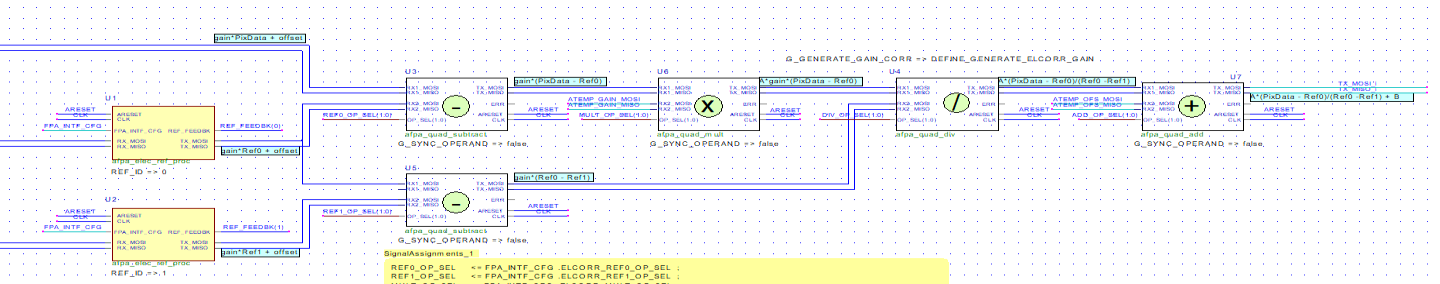
\includegraphics[width=1.2\textwidth]{datapath}
  \caption{Datapath}
  \label{fig:datapath}
\end{figure}

Dans le mode d'opération normal (\texttt{ELCORR\_MODE\_OFFSET\_AND\_GAIN\_CORR}), le datapath calcule donc l'expression suivante:

\[ Y_{out}=A_{gain}\cdot\frac{Y_{pix}-Y_{R1}}{Y_{R1}-Y_{R2}}+A_{offs} \]

Pour plus de flexibilité, les opérateurs du datapath reçoivent un sélecteur d'aiguillage en provenance du processeur qui permet d'implémenter plusieurs modes de calcul différents. Outre le mode normal actif (l'opérateur effectue l'opération mathématique native), on peut sélectionner un mode passage transparent de l'opérande 1 ou passage de l'opérande 2. 

Ainsi, avec la bonne configuration appropriée, on peut demander par exemple au correcteur électronique de passer vers la sortie la REF1 ou la REF2 de manière transparente sans transformation afin de debug. (Cela correspond aux modes \texttt{ELCORR\_MODE\_REF1\_IMG} et \texttt{ELCORR\_MODE\_REF2\_IMG} respectivement.)

\section{Conclusion}
Le correcteur électronique est un module firmware fort utile qui a rendu possible les produits M1k, V500 et M2kUD. Avec sa grande versatilité, il pourra certainement servir pour d'autres détecteurs qui auront besoin d'une compensation active.

\end{document}
